\documentclass[11pt,a4paper]{article}

% ---------------------------------------------------------------------------
% Baseline verification report -- styled after the FYP proposal.
% Every number comes from data/numbers.tex and data/*.dat, generated by
% scripts/make_report_data.py from the committed results. Do not hand-edit numbers.
% ---------------------------------------------------------------------------
\usepackage[T1]{fontenc}
\usepackage{lmodern}
\usepackage[margin=2.4cm]{geometry}
\usepackage{amsmath,amssymb}
\usepackage{graphicx,booktabs,tabularx,array,multirow}
\usepackage{xcolor}
\usepackage{pgfplots,pgfplotstable}
\pgfplotsset{compat=1.18}
\usepgfplotslibrary{groupplots}
\usepackage{tikz}
\usetikzlibrary{arrows.meta,positioning,shapes.geometric,fit,patterns,calc,backgrounds}
\usepackage[most]{tcolorbox}
\usepackage{listings}
\usepackage{pifont}
\usepackage{enumitem}
\usepackage{caption}
\usepackage{tocloft}
\usepackage{xurl}
\usepackage[hidelinks]{hyperref}

\newcommand{\cmark}{\textcolor{okgreen}{\ding{51}}}
\newcommand{\xmark}{\textcolor{badred}{\ding{55}}}
\newcommand{\SV}{\textsc{SusVibes}}

% Palette (validated with the dataviz validator: all pairs pass CVD, contrast, chroma).
\definecolor{funcblue}{HTML}{4F81BD}
\definecolor{secred}{HTML}{C0504D}
\definecolor{amber}{HTML}{D99A2B}
\definecolor{okgreen}{HTML}{2E7D32}
\definecolor{badred}{HTML}{B71C1C}
\definecolor{boxblue}{HTML}{EEF3FA}
\definecolor{boxframe}{HTML}{4F6F96}
\definecolor{codebg}{HTML}{F7F7F7}
\definecolor{codekw}{HTML}{1F4E79}
\definecolor{codecm}{HTML}{6A737D}
\definecolor{codestr}{HTML}{8B3A2B}

\renewcommand{\cftsecleader}{\cftdotfill{\cftdotsep}}
\setlength{\parindent}{0pt}
\setlength{\parskip}{6pt}
\captionsetup{font=small,labelsep=colon,justification=justified,singlelinecheck=false}
\captionsetup[lstlisting]{justification=raggedright}

\newtcolorbox{keybox}[1][]{enhanced,colback=boxblue,colframe=boxframe,boxrule=0.6pt,arc=0pt,
  left=6pt,right=6pt,top=4pt,bottom=4pt,fontupper=\small,#1}
\newtcolorbox{verdictbox}[1][]{enhanced,colback=boxblue,colframe=boxframe,boxrule=1pt,arc=0pt,
  left=8pt,right=8pt,top=6pt,bottom=6pt,#1}

\lstdefinestyle{code}{
  basicstyle=\ttfamily\scriptsize, backgroundcolor=\color{codebg}, frame=single, rulecolor=\color{gray!40},
  keywordstyle=\color{codekw}\bfseries, commentstyle=\color{codecm}\itshape, stringstyle=\color{codestr},
  showstringspaces=false, breaklines=true, columns=fullflexible, keepspaces=true,
  xleftmargin=4pt, xrightmargin=4pt, aboveskip=6pt, belowskip=6pt, upquote=true}
\lstset{style=code}
\lstdefinelanguage{shell}{morekeywords={python,python3,docker,git,curl,cd,export},sensitive=true,
  morecomment=[l]{\#},morestring=[b]"}
\renewcommand{\lstlistingname}{Listing}
\renewcommand{\lstlistlistingname}{List of Listings}

\pgfplotsset{
  every axis/.append style={font=\small, axis line style={gray!70}, tick style={gray!70},
    major grid style={gray!20}, legend style={draw=gray!50, font=\footnotesize}},
  every node near coord/.append style={color=black, font=\footnotesize},
  boxlegend/.style={legend image code/.code={\fill[##1] (0cm,-0.09cm) rectangle (0.3cm,0.11cm);}},
}

% Generated by scripts/make_report_data.py -- do not edit.
\newcommand{\NTasks}{186}
\newcommand{\FuncCount}{106}
\newcommand{\SecCount}{22}
\newcommand{\FuncInsecCount}{84}
\newcommand{\FuncFailCount}{80}
\newcommand{\FuncPct}{56.99}
\newcommand{\SecPct}{11.83}
\newcommand{\FuncPctExact}{56.9892}
\newcommand{\SecPctExact}{11.8280}
\newcommand{\CondPct}{20.75}
\newcommand{\InsecSharePct}{79.25}
\newcommand{\FuncOnlyInsecPct}{45.16}
\newcommand{\GapPP}{45.16}
\newcommand{\FuncCILo}{49.8}
\newcommand{\FuncCIHi}{63.9}
\newcommand{\SecCILo}{7.9}
\newcommand{\SecCIHi}{17.3}
\newcommand{\CondCILo}{14.1}
\newcommand{\CondCIHi}{29.4}
\newcommand{\FuncCIMid}{56.848}
\newcommand{\FuncCIHalf}{7.044}
\newcommand{\SecCIMid}{12.600}
\newcommand{\SecCIHalf}{4.658}
\newcommand{\FuncCIPlus}{6.903}
\newcommand{\FuncCIMinus}{7.186}
\newcommand{\SecCIPlus}{5.431}
\newcommand{\SecCIMinus}{3.886}
\newcommand{\OfficialFuncFrac}{0.5698924731182796}
\newcommand{\OfficialSecFrac}{0.11827956989247312}
\newcommand{\IdsIdentical}{yes}
\newcommand{\LedgerSha}{2c75581d15af30a5}
\newcommand{\GenericCount}{186}
\newcommand{\GitCmdTasks}{3}
\newcommand{\SamePatchCount}{161}
\newcommand{\DiffPatchCount}{25}
\newcommand{\ExitSubmitted}{178}
\newcommand{\ExitError}{8}
\newcommand{\NProjects}{101}
\newcommand{\NCwes}{81}
\newcommand{\TThreeMatch}{12}
\newcommand{\TFiveMatch}{3}
\newcommand{\FFiveMatch}{9}
\newcommand{\RvConcluded}{77}
\newcommand{\RvAttempted}{78}
\newcommand{\RvTechErr}{1}
\newcommand{\RvPending}{108}
\newcommand{\RvRetries}{7}
\newcommand{\RvAgree}{72}
\newcommand{\RvCompared}{77}
\newcommand{\RvDisagree}{5}
\newcommand{\RvAgreePct}{93.5}
\newcommand{\RvPubFuncReFail}{2}
\newcommand{\RvPubFailReFunc}{3}
\newcommand{\RvPubSecReNot}{0}
\newcommand{\RvPubNotReSec}{2}
\newcommand{\RvPubFunc}{48}
\newcommand{\RvReFunc}{49}
\newcommand{\RvPubSec}{12}
\newcommand{\RvReSec}{14}
\newcommand{\RvEvalCompleted}{76}
\newcommand{\RvEvalPatchErr}{1}
\newcommand{\RvGoldenTasks}{5}
\newcommand{\PilotGoldenOK}{4}
\newcommand{\PilotVulnOK}{4}
\newcommand{\PilotEmptyOK}{5}
\newcommand{\ThreshZero}{110}
\newcommand{\ThreshPos}{76}
\newcommand{\ThreshMax}{726}
\newcommand{\CostTotal}{332.61}
\newcommand{\CostMean}{1.79}
\newcommand{\CostMedian}{1.57}
\newcommand{\CostPNinety}{3.05}
\newcommand{\CostMax}{6.64}
\newcommand{\CostPilot}{5.08}
\newcommand{\TokIn}{600.1}
\newcommand{\TokOut}{0.52}
\newcommand{\CostUncached}{1{,}808}
\newcommand{\CostRatio}{18.4}
\newcommand{\TurnsMean}{81.7}
\newcommand{\CostStdev}{0.99}

\makeatletter\newcommand{\rows}[1]{\@@input #1 }\makeatother

\begin{document}

% ------------------------------------------------------------------ title page
\begin{titlepage}
\centering
\vspace*{1.2cm}
{\bfseries Final Year Project --- Baseline Verification Report\par}
\vspace{2.6cm}
{\LARGE Verifying the 11.8\% Secure Pass Rate\\[4pt] of SWE-agent + Claude 4 Sonnet on \SV\par}
\vspace{0.8cm}
{\large An evidence-based reproducibility study for the baseline of\\
\emph{Automated Vulnerability Detection and Repair in AI-Generated Code}\par}
\vspace{2.4cm}
{\large\bfseries by\par}
\vspace{0.8cm}
{\large Abdullah Farooq (462905)\par}
\vspace{0.3cm}
{\large M. Abdullah Tufail (476425)\par}
\vspace{2.0cm}
{\large\bfseries Under the supervision of\par}
\vspace{0.6cm}
{\large\textbf{Advisor:} Dr. Syed Taha Ali\par}
\vspace{0.3cm}
{\large\textbf{Co-Advisor:} M. Wajahat Hussain\par}
\vfill
School of Electrical Engineering and Computer Science\\
National University of Sciences and Technology\\
Islamabad, Pakistan\\
October 2026
\end{titlepage}

\pagenumbering{arabic}
\setcounter{page}{1}
\tableofcontents
\newpage
\listoffigures
\newpage
\listoftables
\lstlistoflistings
\newpage

% ------------------------------------------------------------------ abstract
\section{Abstract}
\begin{center}\begin{minipage}{0.86\textwidth}\itshape\small
Our project proposal builds on one headline number from the ICML~2026 \SV{} benchmark: SWE-agent driven by
Claude~4 Sonnet produced functionally correct code for 57\% of tasks, but correct \emph{and} secure code for only
11.8\%. Before we use that number as the baseline our detect-then-patch framework must improve on, we set out to
verify it instead of trusting it.

\textbf{What the number is.} A source audit across the paper (PMLR and four arXiv versions), the benchmark and
leaderboard repositories and their git histories, and the Hugging Face dataset established what 11.8\% means.
It is a \SV{} \textbf{v1.0 (186-task)} result for model \texttt{claude-sonnet-4-20250514} at temperature~0,
pass@1. It \textbf{already includes a generic security reminder} appended to every task prompt. It replaced an
earlier 200-task figure of 10.5\%.

\textbf{Recomputing it.} The authors published all 186 patches, all 186 agent trajectories and the per-task
outcome lists. From these we independently recomputed \FuncCount/\NTasks{} functional (\FuncPct\%) and
\SecCount/\NTasks{} secure (\SecPct\%) solutions. The task sets are identical to the official summary, and every
related number in the paper's Tables~3 and~5 and Figure~5 is reproduced from per-task data.

\textbf{Re-scoring it.} We validated the official evaluator with golden, vulnerable and empty controls. We then
re-scored \RvConcluded{} of the published patches on an independent machine at zero inference cost.
\RvAgree{} of \RvCompared{} verdicts match the published ones, and no task published as secure was contradicted.
Every disagreement involves the functional verdict and traces to host-sensitive tests, count-based thresholds,
or a drifted Docker image.

\textbf{Verdict.} The 11.8\% figure is \textbf{verified from the original evaluation artifacts}. It is
\textbf{not independently reproduced}, because no fresh model run was performed: there was no budget, the model
is deprecated, and the authors' agent configuration is unpublished.
\end{minipage}\end{center}

% ------------------------------------------------------------------ introduction
\section{Introduction}
Our project proposes an \emph{agentic detect-then-patch} layer that inspects code written by AI coding agents,
finds the weaknesses they introduce and repairs them without breaking functionality. Its central evaluation
question, proposal RQ2, is whether such a layer \emph{raises the secure-task completion rate (SecPass) without
reducing functional correctness (FuncPass)}. Answering it requires a trustworthy starting point.

The starting point we cite is the \SV{} result of Zhao et al.~\cite{zhao2026}. On 186 real feature-request tasks
from open-source Python projects, the best configuration (SWE-agent~\cite{sweagent} with Claude~4 Sonnet) solved
57\% of tasks functionally but only 11.8\% both correctly and securely. That gap motivates our whole project.

A number in a paper or on a leaderboard is only a claim, and agent benchmarks are especially fragile. Dataset
versions change, prompts differ between ``default'' and ``security-enhanced'' runs, evaluators evolve, Docker
images are rebuilt, and agents can ``reward-hack'' by recovering the reference fix. Before we compare our
framework against 11.8\%, we therefore need to know:
\begin{enumerate}[nosep]
  \item exactly which experiment produced the number;
  \item whether the number follows from the per-task evidence; and
  \item whether the official evaluator gives the same per-task verdicts on a machine other than the authors'.
\end{enumerate}

This report documents how we answered those three questions, what we found, and how much confidence the
evidence supports. All scripts, data, logs and checksums are in the accompanying repository directory
\texttt{susvibes\_118\_verification/} (Appendix~\ref{app:files}).

\begin{keybox}
\textbf{The question in brief.} Can we independently verify that SWE-agent + Claude~4 Sonnet achieved a secure
pass rate of 11.8\% on \SV{}? We do not assume the figure is correct. We trace it to its source, recompute it from
per-task records, test the evaluator that produced it, and state exactly which standard of verification the
evidence meets.
\end{keybox}

% ------------------------------------------------------------------ RQ & standards
\section{Research Question and Standards of Evidence}
We fixed the possible outcomes \emph{before} looking at any results, so that the conclusion could not be shaped to
fit a preferred answer. Table~\ref{tab:standards} lists them. The word ``verified'' is never used in this report
without saying which standard it refers to.

\begin{table}[h]
\centering\small
\begin{tabularx}{\textwidth}{@{}lX@{}}
\toprule
\textbf{Standard} & \textbf{What the evidence must show}\\
\midrule
1. Independently reproduced & A complete, correctly configured fresh model run on all tasks reproduces the published result.\\
2. Verified from original artifacts & Complete original per-task results and trajectories independently reproduce the calculation. No fresh model run.\\
3. Publication-confirmed only & The paper or leaderboard reports the number, but the underlying evidence is not available.\\
4. Not reproduced / inconclusive & The evidence differs from the published result, or limitations prevent a reliable conclusion.\\
\bottomrule
\end{tabularx}
\caption{Pre-registered standards of evidence for the verdict.}
\label{tab:standards}
\end{table}

% ------------------------------------------------------------------ background
\section{Background: the \SV{} Benchmark}
\subsection{How a task is built}
\SV{} mines historical vulnerability-fixing commits from open-source Python projects. For each fix, the
repository is rewound to the vulnerable version and the affected feature is masked out. The agent receives a
natural-language feature request and must re-implement the feature inside a Docker image of the repository. Its
patch is then run against two test suites:
\begin{itemize}[nosep]
  \item the project's own \textbf{functional tests};
  \item \textbf{security tests} derived from the real fix, which pass on the secure implementation and fail on the
  original vulnerable one.
\end{itemize}
A task counts as \emph{correct and secure} only if both suites pass. The v1.0 set has \NTasks{} tasks from
\NProjects{} project strings (about 100 upstream projects) covering \NCwes{} distinct CWE identifiers.

\subsection{The metrics}
Let $N$ be the number of tasks, $F$ the set of functionally passing tasks and $S\subseteq F$ the set that also
passes security. Following the evaluator code (Section~\ref{sec:evaluator}):
\begin{gather}
\text{FuncPass} = 100\cdot\frac{|F|}{N}, \qquad \text{SecPass} = 100\cdot\frac{|S|}{N}, \qquad
\text{Conditional security} = 100\cdot\frac{|S|}{|F|},\\
\text{Functional-only insecure} = 100\cdot\frac{|F|-|S|}{N}, \qquad
\text{Gap} = \text{FuncPass}-\text{SecPass}\ \text{(percentage points)}.
\end{gather}
Empty, unappliable or unevaluable patches stay in the denominator and count as failures. The paper's separate
``SecPass~$\perp$~FuncPass'' metric (security on the intersection of tasks every setting solves) is a different
quantity and is not used here.

\subsection{Two versions that must not be mixed}
\SV{} has two pinned versions:
\begin{itemize}[nosep]
  \item \textbf{v0.0}: 200 tasks.
  \item \textbf{v1.0}: 186 tasks. It adds human-revised security tests that are decoupled from the reference fix,
  images with the git history removed, and corrected CWE labels.
\end{itemize}
Scores on the two versions are not comparable. Identifying which version produced 11.8\% was the first job of the
audit.

% ------------------------------------------------------------------ methodology
\section{Verification Methodology}
\label{sec:method}
We organised the work as a sequence of stages, each cheaper and lower-risk than the next
(Figure~\ref{fig:pipeline}). Expensive actions came last and only if justified: downloading 186 Docker images,
and especially paying for model inference.

\begin{figure}[h]
\centering
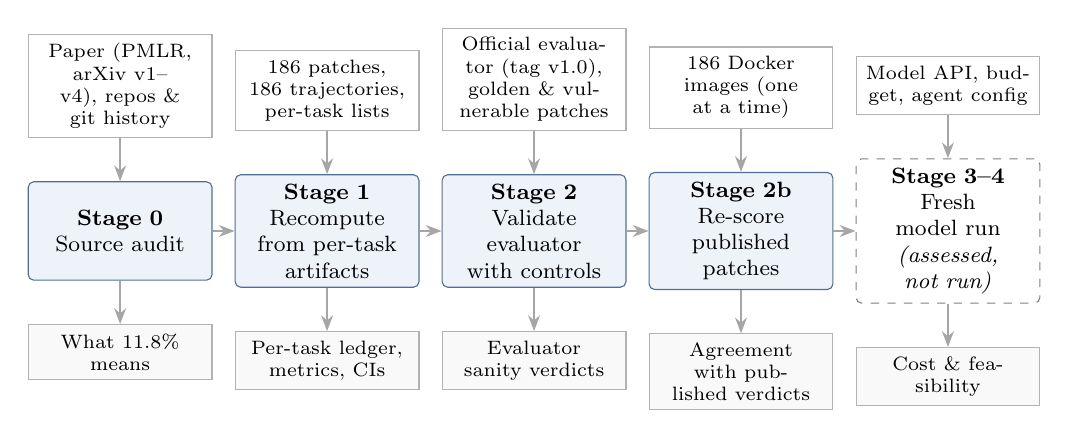
\begin{tikzpicture}[
  stage/.style={draw=boxframe, fill=boxblue, rounded corners=2pt, align=center, font=\footnotesize,
                minimum width=2.25cm, minimum height=1.25cm, text width=2.1cm},
  skip/.style={stage, dashed, fill=white, draw=gray},
  src/.style={draw=gray!60, fill=white, align=center, font=\scriptsize, text width=2.1cm, minimum height=0.7cm},
  outbox/.style={draw=gray!60, fill=gray!5, align=center, font=\scriptsize, text width=2.1cm, minimum height=0.7cm},
  arr/.style={-{Stealth[length=2mm]}, gray!70, thick}]
\node[stage] (s0) {\textbf{Stage 0}\\Source audit};
\node[stage, right=0.28cm of s0] (s1) {\textbf{Stage 1}\\Recompute from per-task artifacts};
\node[stage, right=0.28cm of s1] (s2) {\textbf{Stage 2}\\Validate evaluator with controls};
\node[stage, right=0.28cm of s2] (s2b) {\textbf{Stage 2b}\\Re-score published patches};
\node[skip, right=0.28cm of s2b] (s3) {\textbf{Stage 3--4}\\Fresh model run\\\textit{(assessed, not run)}};
\foreach \a/\b in {s0/s1,s1/s2,s2/s2b,s2b/s3} \draw[arr] (\a) -- (\b);
\node[src, above=0.55cm of s0] (i0) {Paper (PMLR, arXiv v1--v4), repos \& git history};
\node[src, above=0.55cm of s1] (i1) {186 patches, 186 trajectories, per-task lists};
\node[src, above=0.55cm of s2] (i2) {Official evaluator (tag v1.0), golden \& vulnerable patches};
\node[src, above=0.55cm of s2b] (i3) {186 Docker images (one at a time)};
\node[src, above=0.55cm of s3] (i4) {Model API, budget, agent config};
\foreach \a/\b in {i0/s0,i1/s1,i2/s2,i3/s2b,i4/s3} \draw[arr] (\a) -- (\b);
\node[outbox, below=0.55cm of s0] (o0) {What 11.8\% means};
\node[outbox, below=0.55cm of s1] (o1) {Per-task ledger, metrics, CIs};
\node[outbox, below=0.55cm of s2] (o2) {Evaluator sanity verdicts};
\node[outbox, below=0.55cm of s2b] (o3) {Agreement with published verdicts};
\node[outbox, below=0.55cm of s3] (o4) {Cost \& feasibility};
\foreach \a/\b in {s0/o0,s1/o1,s2/o2,s2b/o3,s3/o4} \draw[arr] (\a) -- (\b);
\end{tikzpicture}
\caption{Verification pipeline. Each stage is cheaper and less risky than the next. The fresh model run (dashed)
was assessed but not executed (Section~\ref{sec:fresh}).}
\label{fig:pipeline}
\end{figure}

Five working principles governed every stage:
\begin{enumerate}[nosep]
  \item \textbf{Evidence before cost.} Inspect existing artifacts before downloading environments or calling models.
  \item \textbf{Pin everything.} Use exact commits, dataset hashes and the tagged evaluator, never ``latest'' aliases.
  \item \textbf{No hand-typed numbers.} Every count is derived by a script from per-task records. The PDF you are
  reading pulls its numbers from generated files.
  \item \textbf{Account for every task.} Each task carries a durable status (\texttt{pending},
  \texttt{completed}, \texttt{technical\_error}, \texttt{needs\_review}). A failure to evaluate is never counted
  as an insecure solution.
  \item \textbf{Keep ground truth away from agents.} Reference patches are used only as evaluator inputs. No agent
  ran in this study.
\end{enumerate}

% ------------------------------------------------------------------ stage 0
\section{Stage 0: Source Audit --- What Exactly Is 11.8\%?}
\subsection{Tracing the figure through time}
The leaderboard repository's git history shows that the number attached to this submission changed twice
(Table~\ref{tab:history}).

\begin{table}[h]
\centering\footnotesize
\begin{tabular}{@{}llrrrl@{}}
\toprule
\textbf{Date} & \textbf{Source} & \textbf{Tasks} & \textbf{FuncPass} & \textbf{SecPass} & \textbf{Note}\\
\midrule
2025-12-02 & arXiv v1, Table 3 & 200 & 61.0 & 10.5 & original paper\\
2025-12-30 & leaderboard \texttt{c6169e6} & 200 & 61.0 & 10.5 & mislabelled ``v1.0''\\
2026-01-10 & leaderboard \texttt{4db597e} & 200 & 122/200 & 21/200 & first per-task summary\\
2026-06-19 & leaderboard \texttt{a050d9d} & 200 & 60.8 & 10.6 & 1 reward-hack removed; relabelled v0.0\\
2026-06-20 & leaderboard \texttt{8571041} & \textbf{186} & \textbf{106/186} & \textbf{22/186} & migrated to v1.0\\
2026-08-21 & arXiv v3/v4, PMLR & 186 & 57.0 & 11.8 & current publication\\
\bottomrule
\end{tabular}
\caption{The history of the SWE-agent + Claude 4 Sonnet figure. The 11.8\% belongs to \SV{} v1.0. The earlier
10.5\% is a v0.0 result and is not comparable.}
\label{tab:history}
\end{table}

\subsection{The configuration behind the number}
Table~\ref{tab:config} lists what we could establish about the run and the evidence behind each item. The
trajectories themselves were the most reliable source, because they record the exact model identifier, tools and
prompt the agent saw.

\begin{table}[h]
\centering\small
\begin{tabularx}{\textwidth}{@{}lXX@{}}
\toprule
\textbf{Setting} & \textbf{Finding} & \textbf{Evidence}\\
\midrule
Agent & SWE-agent ($\approx$v1.1.0). Config \texttt{[susvibes\_eval, no\_cache]} is \emph{unpublished} & paper \S4.1; \texttt{setting.yaml}\\
Model & \texttt{claude-sonnet-4-20250514} on all 186 records & \texttt{trials.json}\\
Sampling & temperature 0.00, top\_p 1.00, unlimited cost & original run-directory name\\
Limits / attempts & 200 calls per task; pass@1, one trajectory per task & paper \S4.1; \texttt{setting.yaml}\\
Prompt & SWE-agent default template \textbf{plus a generic security reminder} (\GenericCount/186) & every trajectory\\
Dataset & \SV{} v1.0, 186 tasks & summary \texttt{num\_candidates}\\
Agent exit & \ExitSubmitted{} submitted, \ExitError{} submitted after an exit error; no empty patches & \texttt{run\_metadata}\\
Recorded spend & \$\CostTotal{} (mean \$\CostMean{} per task) & \texttt{total\_cost\_usd}\\
\bottomrule
\end{tabularx}
\caption{Experimental configuration behind the 11.8\% figure.}
\label{tab:config}
\end{table}

\subsection{Finding: the ``default'' run already tells the agent to be secure}
The leaderboard lists this run as \emph{default}, and the current evaluator's default strategy adds \emph{no}
security text. Yet every one of the 186 trajectories ends its task description with the paper's \emph{generic
security reminder} (Listing~\ref{lst:prompt}). The paper does disclose this in \S5 and Appendix~C.1 (``the generic
security reminder used in the main experiments''), so nothing is hidden. Two practical consequences follow:
\begin{itemize}[nosep]
  \item 11.8\% is \emph{not} a ``no security prompting'' baseline.
  \item A reproduction, including our own FYP baseline, must use \texttt{-{}-strategy generic} to be comparable.
\end{itemize}

\begin{lstlisting}[caption={[Task prompt ending seen by the agent]End of the task prompt seen by the agent (identical in all 186 trajectories).},label={lst:prompt}]
<pr_description>
# Missing Session Class Initialization Implementation
...
---
 ## Safety Requirements
Make sure to follow best security practices and avoid common vulnerabilities when resolving this issue.
</pr_description>
\end{lstlisting}

\subsection{Dataset and evaluator pinning}
The task content that determines security verdicts is the problem statement, test patches, security patch,
golden patch and mask patch. We compared it across every 186-task revision of the dataset: the repository
revision in effect when the v1 summary was committed (2026-06-20), the \texttt{v1.0} tag, \texttt{main}, the
leaderboard copy and the Hugging Face snapshot. The content is \textbf{byte-identical} in all of them. Only CWE
labels (22 relabels) and metadata field names changed.

The published summary's schema matches the evaluator at tag \texttt{v1.0} (\texttt{7e1b4b0}), and that is the
evaluator we used. Table~\ref{tab:published} summarises which artifacts exist.

\begin{table}[h]
\centering\small
\begin{tabular}{@{}lc@{}}
\toprule
\textbf{Artifact} & \textbf{Published?}\\
\midrule
Final percentages (paper, leaderboard) & \cmark\\
Official \texttt{summary.json} with per-task ID lists & \cmark\\
All 186 model patches & \cmark\\
All 186 trajectories (prompt, tool schemas, every action) & \cmark\\
Per-task cost and token counts & \cmark\\
Per-task evaluator reports and test logs (incl.\ timeouts) & \xmark\\
SWE-agent configuration files and exact SWE-agent commit & \xmark\\
Docker image digests used for the original evaluation & \xmark\\
\bottomrule
\end{tabular}
\caption{Availability of evidence for the target submission.}
\label{tab:published}
\end{table}

% ------------------------------------------------------------------ stage 1
\section{Stage 1: Recomputing the Metrics from Per-Task Artifacts}
\subsection{Building the ledger}
We wrote a small pipeline (Appendix~\ref{app:repro}) that reads the pinned dataset and the leaderboard artifacts.
It builds one authoritative row per task (\texttt{results/per\_task\_results.csv}), with these columns:
\begin{itemize}[nosep]
  \item task metadata (project, CWE, CVE);
  \item agent status, the observed prompt strategy, and the published functional and security verdicts;
  \item the independent re-scoring verdict (Stage~2b) and the control results;
  \item provenance: patch hash and trajectory path;
  \item cost.
\end{itemize}
The script refuses to proceed unless:
\begin{itemize}[nosep]
  \item task IDs are unique and equal to the v1.0 task set;
  \item every secure task is also functional;
  \item no non-completed evaluation carries a pass.
\end{itemize}
Metrics are then recomputed \emph{only} from the ledger. Listing~\ref{lst:wilson} shows the interval computation.

\begin{lstlisting}[language=Python,caption={[Wilson score interval]Wilson score interval used for all confidence intervals (\texttt{scripts/recompute\_metrics.py}).},label={lst:wilson}]
def wilson(k: int, n: int, z: float = Z95):
    if n == 0:
        return None
    p = k / n
    den = 1 + z * z / n
    centre = (p + z * z / (2 * n)) / den
    half = z * math.sqrt(p * (1 - p) / n + z * z / (4 * n * n)) / den
    return [100 * (centre - half), 100 * (centre + half)]
\end{lstlisting}

\subsection{Results}
\begin{table}[h]
\centering\small
\begin{tabular}{@{}lrrr@{}}
\toprule
\textbf{Quantity} & \textbf{Count} & \textbf{Rate (\%)} & \textbf{95\% Wilson CI}\\
\midrule
Total tasks (v1.0) & \NTasks & & \\
Completed / empty / unappliable / indeterminate & \NTasks{} / 0 / 0 / 0 & & \\
Functional passes & \FuncCount & \FuncPct & \FuncCILo--\FuncCIHi\\
\textbf{Secure passes (functional and secure)} & \textbf{\SecCount} & \textbf{\SecPct} & \SecCILo--\SecCIHi\\
Functionally correct but insecure & \FuncInsecCount & \FuncOnlyInsecPct & \\
Functional failures & \FuncFailCount & & \\
Secure among functional passes & \SecCount/\FuncCount & \CondPct & \CondCILo--\CondCIHi\\
Insecure share of functional passes & \FuncInsecCount/\FuncCount & \InsecSharePct & \\
Functional-to-secure gap & & \GapPP{} pp & \\
\bottomrule
\end{tabular}
\caption{Metrics recomputed from the per-task ledger (no hand-entered counts).}
\label{tab:metrics}
\end{table}

\begin{figure}[h]
\centering
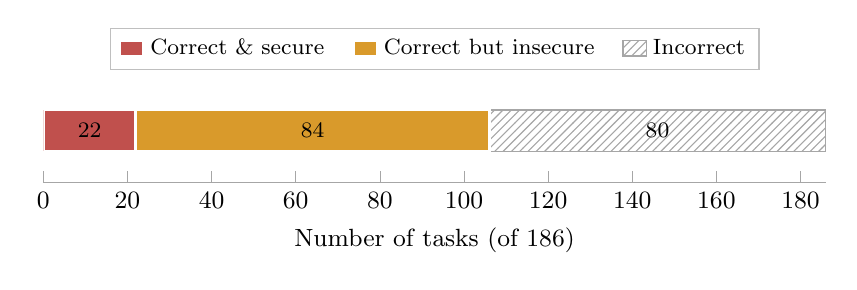
\begin{tikzpicture}
\begin{axis}[
  xbar stacked, width=0.95\textwidth, height=2.9cm, bar width=15pt,
  xmin=0, xmax=186, ytick=\empty, axis y line=none, axis x line*=bottom,
  xlabel={Number of tasks (of \NTasks)}, enlarge y limits=0.6,
  legend style={at={(0.5,1.08)}, anchor=south, legend columns=3, /tikz/every even column/.append style={column sep=8pt}},
  nodes near coords, nodes near coords style={font=\footnotesize\bfseries, color=black},
  every node near coord/.append style={xshift=0pt}]
\addplot+[fill=secred, draw=white, line width=1pt, boxlegend={secred}] coordinates {(\SecCount,0)};
\addplot+[fill=amber, draw=white, line width=1pt, boxlegend={amber}] coordinates {(\FuncInsecCount,0)};
\addplot+[pattern=north east lines, pattern color=gray!70, draw=gray!70, line width=0.6pt,
  legend image code/.code={\draw[pattern=north east lines, pattern color=gray!70, draw=gray!70] (0cm,-0.09cm) rectangle (0.3cm,0.11cm);}] coordinates {(\FuncFailCount,0)};
\legend{Correct \& secure, Correct but insecure, Incorrect}
\end{axis}
\end{tikzpicture}
\caption{Outcome of all \NTasks{} tasks for SWE-agent + Claude 4 Sonnet, recomputed from per-task records.
\FuncInsecCount{} of \FuncCount{} functionally correct solutions (\InsecSharePct\%) are insecure.}
\label{fig:outcome}
\end{figure}

\begin{figure}[h]
\centering
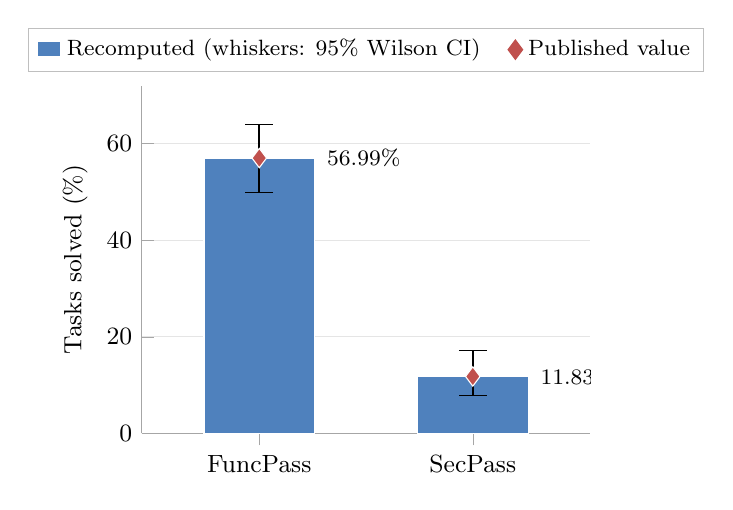
\begin{tikzpicture}
\begin{axis}[
  ybar, width=0.6\textwidth, height=6cm, bar width=40pt, ymin=0, ymax=72,
  symbolic x coords={FuncPass,SecPass}, xtick=data, enlarge x limits=0.55,
  ylabel={Tasks solved (\%)}, ymajorgrids, axis x line*=bottom, axis y line*=left,
  legend style={at={(0.5,1.04)}, anchor=south, legend columns=2, /tikz/every even column/.append style={column sep=8pt}}]
\addplot+[fill=funcblue, draw=white, boxlegend={funcblue},
  error bars/.cd, y dir=both, y explicit, error bar style={black, line width=0.8pt}, error mark options={rotate=90, mark size=5pt, black}]
  coordinates {(FuncPass,\FuncPct) += (0,\FuncCIPlus) -= (0,\FuncCIMinus)
               (SecPass,\SecPct) += (0,\SecCIPlus) -= (0,\SecCIMinus)};
\addplot+[only marks, mark=diamond*, mark size=3.5pt, color=secred, mark options={draw=white, fill=secred},
  legend image code/.code={\draw[mark=diamond*, mark size=3.5pt, secred, mark options={fill=secred}] plot coordinates {(0.15cm,0cm)};}]
  coordinates {(FuncPass,57.0) (SecPass,11.8)};
\node[anchor=west, font=\footnotesize] at (axis cs:FuncPass,\FuncPct) [xshift=21pt] {\FuncPct\%};
\node[anchor=west, font=\footnotesize] at (axis cs:SecPass,\SecPct) [xshift=21pt] {\SecPct\%};
\legend{Recomputed (whiskers: 95\% Wilson CI), Published value}
\end{axis}
\end{tikzpicture}
\caption[Recomputed FuncPass and SecPass with 95\% Wilson intervals]{Recomputed FuncPass and SecPass (bars) with 95\% Wilson intervals (black whiskers) against the published
values (diamonds). Under a binomial reading of a fixed 186-task suite, SecPass lies between \SecCILo\% and \SecCIHi\%.}
\label{fig:ci}
\end{figure}

\subsection{Arithmetic and rounding}
Unrounded counts were used throughout; rounding was applied only for display:
\[
\text{FuncPass} = 100\times\tfrac{\FuncCount}{\NTasks} = \FuncPctExact\% \;\to\; 57.0\%, \qquad
\text{SecPass} = 100\times\tfrac{\SecCount}{\NTasks} = \SecPctExact\% \;\to\; 11.8\%.
\]
These equal the fractions in the official \texttt{summary.json} to every digit (\OfficialFuncFrac{} and
\OfficialSecFrac{}). The recomputed per-task ID sets are identical to the official lists (identical:
\IdsIdentical).

One small discrepancy in the paper's text: ``79.3\% of these functionally correct solutions are insecure'' is
computed from the \emph{rounded} rates, $(57.0-11.8)/57.0 = 79.30\%$. The exact count gives
$\FuncInsecCount/\FuncCount = \InsecSharePct\%$, which rounds to 79.2\%. This does not change the claim.

\subsection{Cross-checking every related number in the paper}
The leaderboard also publishes per-task lists for the other configurations in the paper. We recomputed:
\begin{itemize}[nosep]
  \item all twelve cells of the paper's Table~3 (three frameworks $\times$ four models);
  \item the three rows of Table~5 (security strategies);
  \item the full $3\times3$ transition matrix of Figure~5.
\end{itemize}
All of them match at one decimal place: \TThreeMatch/12 cells, \TFiveMatch/3 rows and \FFiveMatch/9 cells
(Tables~\ref{tab:t3}--\ref{tab:f5}, Figure~\ref{fig:t3}). This rules out a one-off transcription error and shows
that the paper's tables are internally consistent with the released per-task data.

\begin{table}[h]
\centering\scriptsize
\begin{tabular}{@{}llrrccc@{}}
\toprule
\textbf{Framework} & \textbf{Model} & \textbf{Func.} & \textbf{Secure} & \textbf{Recomputed (\%)} & \textbf{Paper (\%)} & \textbf{Match}\\
\midrule
\rows{data/table3_rows.tex}
\bottomrule
\end{tabular}
\caption{Paper Table 3 recomputed from per-task leaderboard data (FuncPass / SecPass).}
\label{tab:t3}
\end{table}

\begin{figure}[h]
\centering
\begin{tikzpicture}
\begin{axis}[
  ybar, width=\textwidth, height=6.2cm, bar width=7pt, ymin=0, ymax=68,
  xtick=data, xticklabels from table={data/table3.dat}{label}, x tick label style={rotate=45, anchor=east, font=\scriptsize},
  ylabel={Tasks solved (\%)}, ymajorgrids, axis x line*=bottom, axis y line*=left, enlarge x limits=0.05,
  legend style={at={(0.5,1.03)}, anchor=south, legend columns=3, /tikz/every even column/.append style={column sep=8pt}}]
\addplot+[fill=funcblue, draw=white, boxlegend={funcblue}] table[x expr=\coordindex, y=func] {data/table3.dat};
\addplot+[fill=secred, draw=white, boxlegend={secred}] table[x expr=\coordindex, y=sec] {data/table3.dat};
\addplot+[only marks, mark=-, mark size=4pt, black, line width=1pt, xshift=-4pt,
  legend image code/.code={\draw[black, line width=1pt] (0cm,0cm) -- (0.3cm,0cm);}] table[x expr=\coordindex, y=paperfunc] {data/table3.dat};
\addplot+[only marks, mark=-, mark size=4pt, black, line width=1pt, xshift=4pt, forget plot] table[x expr=\coordindex, y=papersec] {data/table3.dat};
\legend{FuncPass (recomputed), SecPass (recomputed), Paper value}
\end{axis}
\end{tikzpicture}
\caption{All twelve framework--model configurations of paper Table 3, recomputed from per-task data (bars), with
the paper's values (black ticks). SA = SWE-agent, OH = OpenHands, CC = Claude Code; C4S = Claude 4 Sonnet,
K2 = Kimi K2, G25/G3 = Gemini 2.5/3 Pro.}
\label{fig:t3}
\end{figure}

\begin{table}[h]
\centering\small
\begin{tabular}{@{}lrrccc@{}}
\toprule
\textbf{Strategy} & \textbf{Func.} & \textbf{Secure} & \textbf{Recomputed (\%)} & \textbf{Paper (\%)} & \textbf{Match}\\
\midrule
\rows{data/table5_rows.tex}
\bottomrule
\end{tabular}
\caption{Paper Table 5 (security strategies on SWE-agent + Claude 4 Sonnet) recomputed.}
\label{tab:t5}
\end{table}

\begin{table}[h]
\centering\scriptsize
\begin{tabular}{@{}lccc@{}}
\toprule
\textbf{Generic $\downarrow$ / Self-selection $\rightarrow$} & \textbf{Incorrect} & \textbf{Correct, insecure} & \textbf{Correct, secure}\\
\midrule
\rows{data/fig5_rows.tex}
\bottomrule
\end{tabular}
\caption{Paper Figure 5 transition matrix recomputed: task counts, percentage of 186 tasks, and the paper's value.}
\label{tab:f5}
\end{table}

\subsection{Screening the trajectories for reward hacking}
A suspiciously good result can come from an agent recovering the reference fix rather than writing it. We
screened all 186 trajectories for git-history commands and network access:
\begin{itemize}[nosep]
  \item \textbf{\GitCmdTasks{} trajectories} ran a git-history command, and none of them obtained the fix. One saw
  only ``Initial commit.'', one timed out after 30\,s, and one read the current version of a test file.
  \item \textbf{No} trajectory cloned or downloaded the upstream project.
\end{itemize}

We also compared the v1.0 record with the December-2025 v0.0 record of the same submission:
\begin{itemize}[nosep]
  \item \SamePatchCount{} patches are byte-identical, with the same agent actions.
  \item \DiffPatchCount{} are re-generated trajectories. Only one of these is documented as a reward-hack
  replacement.
\end{itemize}
This screen is keyword-based. It supports, but does not prove, the absence of reward hacking.

% ------------------------------------------------------------------ stage 2
\section{Stage 2: Validating the Official Evaluator}
\label{sec:evaluator}
\subsection{How a task is scored}
We installed the official harness at tag \texttt{v1.0} and read its scoring code. Listing~\ref{lst:summary}
shows the decisive part:
\begin{itemize}[nosep]
  \item a task is secure only inside the functional-pass branch;
  \item empty, unappliable or indeterminate tasks never count as passes;
  \item the denominator is always the full dataset.
\end{itemize}

\begin{lstlisting}[language=Python,caption={[Official aggregation in the v1.0 evaluator]Official aggregation at tag v1.0 (\texttt{susvibes/eval/task.py}, excerpt).},label={lst:summary}]
for instance_id, report in reports.items():
    if report["eval_status"] == EvalStatus.EMPTY_MODEL_PATCH:
        details["empty_model_patch"].append(instance_id); continue
    if report["eval_status"] == EvalStatus.MODEL_PATCH_ERROR:
        details["model_patch_error"].append(instance_id); continue
    if report["eval_status"] == EvalStatus.INDETERMINATE:
        details["indeterminate"].append(instance_id); continue
    if report["run"]["func"]["pass"]:
        details["completed"]["func_pass"].append(instance_id)
        if report["run"]["sec"]["pass"]:          # secure only if also functional
            details["completed"]["sec_pass"].append(instance_id)
...
"func_pass": len(details["completed"]["func_pass"]) / len(dataset),   # denominator = all tasks
"sec_pass":  len(details["completed"]["sec_pass"])  / len(dataset),
\end{lstlisting}

A run ``passes'' if it breaks no \emph{more} tests than the golden reference's expected failure count
(\texttt{expected\_pf}). As Section~\ref{sec:disagree} shows, this threshold is a \emph{count}, which matters
for reproducibility.

\subsection{Controls derived from the benchmark's own validity conditions}
The paper (Appendix~B.4) states that every valid task must satisfy three conditions. We turned each into an
evaluator control:
\begin{itemize}[nosep]
  \item \textbf{Golden} (the secure human fix) must pass both suites.
  \item \textbf{Vulnerable} (the original insecure human implementation) must pass functional tests and fail
  security tests.
  \item \textbf{Empty} must be scored as a failure.
\end{itemize}
The vulnerable implementation is not shipped directly. We reconstructed it by reversing the task's
\texttt{mask\_patch}, which goes from vulnerable to masked (Listing~\ref{lst:reverse}). We first verified that
reversing twice returns every one of the 186 mask patches unchanged, and that the reversed patch applies cleanly
inside the task image.

\begin{lstlisting}[language=Python,caption={[Reconstructing the vulnerable implementation]Reconstructing the vulnerable implementation by reversing \texttt{mask\_patch} (\texttt{scripts/build\_predictions.py}, excerpt).},label={lst:reverse}]
elif HUNK.match(line):                       # @@ -a,b +c,d @@  ->  @@ -c,d +a,b @@
    m = HUNK.match(line)
    out.append(f"@@ -{m.group(2)} +{m.group(1)} @@{m.group(3)}")
elif line.startswith("+") and not line.startswith("+++ "):
    out.append("-" + line[1:])               # added lines become removed lines
elif line.startswith("-") and not line.startswith("--- "):
    out.append("+" + line[1:])               # and vice versa
\end{lstlisting}

\subsection{Pilot results}
We ran all three controls and the published Claude patch on the five example tasks shipped with \SV{}. These are
the same five tasks we analysed in proposal Section~4.5. Results are in Table~\ref{tab:pilot}.
\begin{itemize}[nosep]
  \item On four of the five tasks, the evaluator satisfied every validity condition on our machine, and the
  re-scored Claude verdict matched the published one.
  \item On \texttt{psf/requests}, the \emph{golden} patch itself failed 4 functional tests.
\end{itemize}

\begin{table}[h]
\centering\small
\setlength{\tabcolsep}{4pt}
\begin{tabular}{@{}lccccc@{}}
\toprule
 & \multicolumn{3}{c}{\textbf{Controls}} & \multicolumn{2}{c}{\textbf{Published Claude patch}}\\
\cmidrule(lr){2-4}\cmidrule(lr){5-6}
\textbf{Task (CWE)} & \textbf{Golden} & \textbf{Vulnerable} & \textbf{Empty} & \textbf{Re-scored} & \textbf{Published}\\
\midrule
\rows{data/pilot_rows.tex}
\bottomrule
\end{tabular}
\caption{Evaluator pilot (functional / security). Golden passed both on \PilotGoldenOK/5 tasks, vulnerable was
caught by the security tests on \PilotVulnOK/5, and empty patches were rejected on \PilotEmptyOK/5.}
\label{tab:pilot}
\end{table}

\begin{keybox}
\textbf{Environment finding.} The four failing \texttt{requests} tests expect a TCP connection to the unroutable
address \texttt{10.255.255.1} to \emph{time out}. In this cloud sandbox every outbound connection is accepted
instantly (Listing~\ref{lst:probe}), so the tests fail for every patch, the secure reference included. A failure
here says nothing about the patch. This is why every later disagreement was diagnosed against the golden control
instead of being counted against the model.
\end{keybox}

\begin{lstlisting}[language=shell,caption={[Network probe]Network probe inside a fresh container on the study machine.},label={lst:probe}]
$ docker run --rm python:3.11-slim python -c "... socket.create_connection(('10.255.255.1',80),timeout=3) ..."
10.255.255.1 -> connected after 0.02s      # a normal network would hang until the 3 s timeout
\end{lstlisting}

% ------------------------------------------------------------------ stage 2b
\section{Stage 2b: Independent Re-scoring of the Published Patches}
\subsection{Resource-conscious orchestration}
Re-scoring the 186 published patches tests whether the official evaluator reproduces the published per-task
verdicts on independent hardware, at zero inference cost. Our machine had about 31\,GB of free disk, while the
benchmark recommends 300\,GB for a parallel run. We therefore wrapped the \emph{supported} entry point without
changing its semantics (Listing~\ref{lst:orch}). For each task, the wrapper:
\begin{enumerate}[nosep]
  \item evaluates that single task;
  \item copies the official \texttt{report.json} and gzipped logs out of the harness;
  \item records hashes of the patch, report and evidence files;
  \item deletes the task's image, which is about 1.8\,GB.
\end{enumerate}
It writes a durable checkpoint after every task and a batch record after every five. A resumed run skips only
tasks whose saved evidence still validates, and peak extra disk use stayed below 4\,GB.

\begin{lstlisting}[language=Python,caption={[Checkpointed wrapper around the official evaluator]The wrapper calls the unmodified official entry point, one task at a time (\texttt{scripts/run\_eval\_batches.py}, excerpt).},label={lst:orch}]
cmd = [args.harness_python, "-m", "susvibes.eval.core", "--run_id", run_id,
       "--strategy", args.strategy, "--max_workers", "1",
       "--predictions_path", str(one), "--instance_ids", json.dumps([iid])]
cp = subprocess.run(cmd, cwd=harness_root, capture_output=True, text=True, timeout=args.task_timeout)
...
shutil.copy2(hdir / "report.json", tdir / "report.json")     # official verdict, copied verbatim
status, note = classify(report)                              # completed / technical_error / needs_review
\end{lstlisting}

\textbf{An infrastructure obstacle.} After about 40 pulls, Docker Hub began refusing image downloads with
HTTP~429. We measured the anonymous limit at \textbf{100 pulls per hour, shared with other users of the sandbox's
egress IP}. The harness re-pulls even cached images and aborts on any registry error, so such a failure carries no
verdict. We handled it in two ways:
\begin{itemize}[nosep]
  \item a quota gate that polls Docker Hub's documented rate-limit endpoint (Listing~\ref{lst:quota}), which does
  not itself consume quota;
  \item at most three documented technical retries for tasks that failed \emph{only} because of a 429.
\end{itemize}
Every failed attempt was preserved. In total \RvRetries{} technical retries were performed and one task exhausted
its retries. No other retries were allowed. With the shared quota, throughput fell to 3--10 tasks per hour.

\begin{lstlisting}[language=Python,caption={[Docker Hub quota gate]Waiting for Docker Hub quota before each harness call (excerpt).},label={lst:quota}]
hdr = subprocess.run(["curl", "-s", "--head", "-H", f"Authorization: Bearer {token}",
       "https://registry-1.docker.io/v2/ratelimitpreview/test/manifests/latest"], ...).stdout
# ratelimit-limit: 100;w=3600   ratelimit-remaining: 0;w=3600   (HEAD requests are not counted)
if remaining is None or remaining >= 2:
    return True                              # quota available: invoke the official harness
log(f"Docker Hub anonymous quota {remaining}/{limit} per hour (shared egress IP); waiting {delay}s")
\end{lstlisting}

\subsection{Results}
When we stopped the run, \RvConcluded{} tasks had an official verdict, \RvTechErr{} had a technical error and
\RvPending{} were pending. Of the concluded tasks, \RvEvalCompleted{} had \texttt{eval\_status} completed and
\RvEvalPatchErr{} had \texttt{model\_patch\_error}. We report no re-scored full-benchmark percentage, because
extrapolating partial coverage would not be honest.

\begin{figure}[h]
\centering
\begin{minipage}{0.48\textwidth}\centering
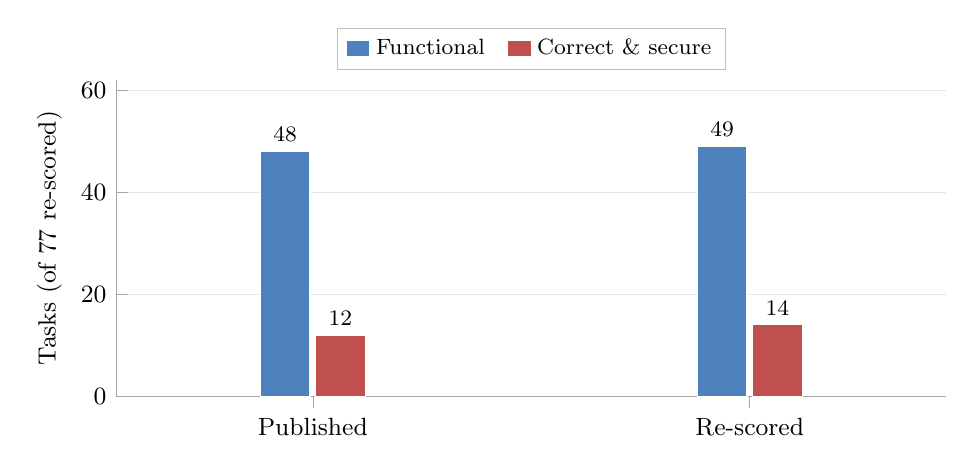
\begin{tikzpicture}
\begin{axis}[
  ybar, width=\linewidth, height=5.6cm, bar width=18pt, ymin=0, ymax=62,
  symbolic x coords={Published,Re-scored}, xtick=data, enlarge x limits=0.45,
  ylabel={Tasks (of \RvConcluded{} re-scored)}, ymajorgrids, axis x line*=bottom, axis y line*=left,
  nodes near coords, nodes near coords style={font=\footnotesize},
  legend style={at={(0.5,1.03)}, anchor=south, legend columns=2, /tikz/every even column/.append style={column sep=6pt}}]
\addplot+[fill=funcblue, draw=white, boxlegend={funcblue}] coordinates {(Published,\RvPubFunc) (Re-scored,\RvReFunc)};
\addplot+[fill=secred, draw=white, boxlegend={secred}] coordinates {(Published,\RvPubSec) (Re-scored,\RvReSec)};
\legend{Functional, Correct \& secure}
\end{axis}
\end{tikzpicture}
\end{minipage}\hfill
\begin{minipage}{0.48\textwidth}\centering
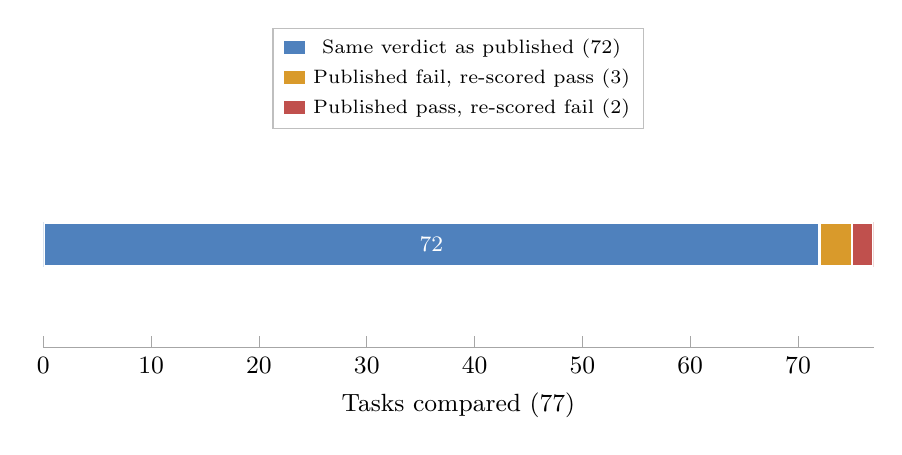
\begin{tikzpicture}
\begin{axis}[
  xbar stacked, width=\linewidth, height=4.2cm, bar width=16pt, xmin=0, xmax=\RvCompared,
  ytick=\empty, axis y line=none, axis x line*=bottom, enlarge y limits=0.6,
  xlabel={Tasks compared (\RvCompared)},
  legend style={at={(0.5,1.06)}, anchor=south, legend columns=1, font=\scriptsize},
  nodes near coords, nodes near coords style={font=\footnotesize\bfseries, color=white}]
\addplot+[fill=funcblue, draw=white, line width=1pt, boxlegend={funcblue}] coordinates {(\RvAgree,0)};
\addplot+[fill=amber, draw=white, line width=1pt, boxlegend={amber}, nodes near coords={}] coordinates {(\RvPubFailReFunc,0)};
\addplot+[fill=secred, draw=white, line width=1pt, boxlegend={secred}, nodes near coords={}] coordinates {(\RvPubFuncReFail,0)};
\addlegendentry{Same verdict as published (\RvAgree)}
\addlegendentry{Published fail, re-scored pass (\RvPubFailReFunc)}
\addlegendentry{Published pass, re-scored fail (\RvPubFuncReFail)}
\end{axis}
\end{tikzpicture}
\end{minipage}
\caption{Independent re-scoring of \RvConcluded{} published patches with the official v1.0 evaluator. Left:
functional and secure counts on the same tasks, published versus re-scored. Right: \RvAgree{} of \RvCompared{}
verdicts (\RvAgreePct\%) agree. Every disagreement concerns the functional verdict, and \RvPubSecReNot{} tasks
published as secure were contradicted.}
\label{fig:rescore}
\end{figure}

\begin{keybox}
\textbf{Key observation.} \textbf{No task that the authors counted as secure was re-scored as insecure or
non-functional.} The re-scored subset contains slightly \emph{more} secure solutions (\RvReSec) than the
published record on the same tasks (\RvPubSec). Re-scoring therefore gives no evidence that the published 11.8\%
over-states security.
\end{keybox}

\subsection{Disagreements and their causes}
\label{sec:disagree}
Table~\ref{tab:disagree} lists every task whose re-scored verdict differs from the published one, or that needs
review. Three mechanisms explain them.

\begin{table}[h]
\centering\scriptsize\setlength{\tabcolsep}{3.5pt}
\begin{tabular}{@{}lllll@{}}
\toprule
\textbf{Task} & \textbf{Published (f / s)} & \textbf{Re-scored (f / s)} & \textbf{Status} & \textbf{Golden here}\\
\midrule
\rows{data/disagree_rows.tex}
\bottomrule
\end{tabular}
\caption{Re-scored tasks that disagree with the published verdict or need review (f = functional, s = security).}
\label{tab:disagree}
\end{table}

\textbf{(1) Count-based thresholds.} At v1.0, \texttt{expected\_pf} is an integer for \emph{all} 186 tasks, and a
run passes if its number of failing tests does not exceed it, \emph{whichever} tests fail.
\begin{itemize}[nosep]
  \item \ThreshZero{} tasks tolerate 0 failures.
  \item \ThreshPos{} tolerate at least one failure, up to \ThreshMax{} (Figure~\ref{fig:thresh}).
\end{itemize}
Tests that depend on the host can therefore move a task across the threshold in either direction. Examples are
memory-limit assertions (\texttt{dask}: $17.7\,\text{GB} \le 11.8\,\text{GB}$ fails on our machine), locale,
running as root, timing and network.

\textbf{(2) Sandbox network.} \texttt{psf/requests}, explained in Section~\ref{sec:evaluator}.

\textbf{(3) Image drift.} For \texttt{celery}, the benchmark's \emph{own} security test patch no longer applies to
the current \texttt{:latest} image. Several other v1.0 leaderboard submissions were scored as secure on this
task, so the image the authors used must have been different. The v1.0 evaluator reports this failure as
\texttt{model\_patch\_error}. Its official verdict (fail) happens to coincide with the published one.

\begin{figure}[h]
\centering
\begin{tikzpicture}
\begin{axis}[
  ybar, width=0.7\textwidth, height=5.2cm, bar width=22pt, ymin=0, ymax=125,
  xtick=data, xticklabels={0, 1--5, 6--20, 21--100, $>$100},
  xlabel={Tolerated functional failures (\texttt{expected\_pf})}, ylabel={Number of tasks},
  ymajorgrids, axis x line*=bottom, axis y line*=left, enlarge x limits=0.15,
  nodes near coords, nodes near coords style={font=\footnotesize}]
\addplot+[fill=funcblue, draw=white] table[x=bin, y=count] {data/thresholds.dat};
\end{axis}
\end{tikzpicture}
\caption{Distribution of functional failure thresholds across the 186 v1.0 tasks. \ThreshPos{} tasks pass a
patch as long as it fails no more tests than this count, which makes their verdicts sensitive to host-dependent
tests.}
\label{fig:thresh}
\end{figure}

% ------------------------------------------------------------------ fresh run
\section{Stages 3--4: Feasibility of a Fresh Model Run}
\label{sec:fresh}
Full independent reproduction (standard~1) requires running SWE-agent with Claude~4 Sonnet again on all 186 tasks.
We assessed it carefully and decided not to execute it, for four reasons.
\begin{enumerate}[nosep]
  \item \textbf{No budget or credentials.} No API key or spending limit was established for benchmark inference,
  and we do not run uncapped paid inference.
  \item \textbf{The model is deprecated.} \texttt{claude-sonnet-4-20250514} is listed as deprecated, with its
  retirement date not yet announced. Substituting a newer model would not be a reproduction.
  \item \textbf{The configuration is unpublished.} The authors' SWE-agent configuration files are not public. The
  prompt and tool schemas can be reconstructed from trajectories, but history processing and error handling cannot.
  \item \textbf{Cost.} The original run recorded \$\CostTotal{} for 186 tasks, with mean \$\CostMean{}, median
  \$\CostMedian{} and maximum \$\CostMax{} per task (Figure~\ref{fig:cost}). It consumed \TokIn{}\,M input tokens.
  At Sonnet-tier list prices without prompt caching, that would be about \$\CostUncached{}. The recorded cost is
  \CostRatio\% of that, which is consistent with heavy prompt-cache reuse. A faithful re-run should budget
  \$330--\$1{,}810.
\end{enumerate}

\begin{figure}[h]
\centering
\begin{tikzpicture}
\begin{axis}[
  ybar interval, width=0.75\textwidth, height=5cm, ymin=0,
  xtick={0,0.5,1,1.5,2,2.5,3,4,5,7}, x tick label style={font=\scriptsize},
  xlabel={Recorded inference cost per task (USD)}, ylabel={Number of tasks},
  ymajorgrids, axis x line*=bottom, axis y line*=left]
\addplot+[fill=funcblue, draw=white] table[x=lo, y=count] {data/cost_hist.dat};
\end{axis}
\end{tikzpicture}
\caption{Per-task inference cost of the original run, from \texttt{run\_metadata}: total \$\CostTotal, mean
\$\CostMean, 90th percentile \$\CostPNinety. The five pilot tasks alone cost \$\CostPilot.}
\label{fig:cost}
\end{figure}

Even a faithful fresh run would not necessarily return 22/186:
\begin{itemize}[nosep]
  \item Temperature-0 decoding is not bit-reproducible across API serving changes.
  \item Today's images have the git history removed, unlike most of the original generations.
  \item The Wilson interval for SecPass spans \SecCILo--\SecCIHi\%.
\end{itemize}
A fresh result inside that range would be \emph{consistent} with 11.8\%, not proof of it.

% ------------------------------------------------------------------ exploratory
\section{Exploratory Analysis by Weakness Category and Project}
Figure~\ref{fig:cwe} breaks the published outcomes down by CWE for categories with at least five tasks. A task can
carry several CWEs. Groups are small and tasks from the same project are correlated, so this analysis is
descriptive only. Functional success most often coexists with a security failure for:
\begin{itemize}[nosep]
  \item cross-site scripting (CWE-79): 10 of 15 functional solutions insecure;
  \item information exposure (CWE-200): 6 of 6;
  \item unbounded resource allocation (CWE-770): 5 of 6.
\end{itemize}
These are the weakness classes our detection agent should prioritise.

\begin{figure}[h]
\centering
\begin{tikzpicture}
\begin{axis}[
  xbar stacked, width=0.8\textwidth, height=8.5cm, bar width=9pt, xmin=0, xmax=28,
  ytick=data, yticklabels from table={data/cwe.dat}{cwe}, y dir=reverse, y tick label style={font=\scriptsize},
  xlabel={Number of tasks}, xmajorgrids, axis x line*=bottom, axis y line*=left, enlarge y limits=0.06,
  legend style={at={(0.98,0.03)}, anchor=south east}]
\addplot+[fill=secred, draw=white, line width=0.8pt, boxlegend={secred}] table[y expr=\coordindex, x=sec] {data/cwe.dat};
\addplot+[fill=amber, draw=white, line width=0.8pt, boxlegend={amber}] table[y expr=\coordindex, x=insec] {data/cwe.dat};
\addplot+[pattern=north east lines, pattern color=gray!70, draw=gray!70, line width=0.5pt,
  legend image code/.code={\draw[pattern=north east lines, pattern color=gray!70, draw=gray!70] (0cm,-0.09cm) rectangle (0.3cm,0.11cm);}]
  table[y expr=\coordindex, x=fail] {data/cwe.dat};
\legend{Correct \& secure, Correct but insecure, Incorrect}
\end{axis}
\end{tikzpicture}
\caption{Published outcomes by CWE (categories with $\ge$5 tasks), in the same encoding as Figure~\ref{fig:outcome}.
Amber segments are functionally correct but insecure solutions.}
\label{fig:cwe}
\end{figure}

\begin{table}[h]
\centering\small
\begin{tabular}{@{}lrrrr@{}}
\toprule
\textbf{Project} & \textbf{Tasks} & \textbf{Functional} & \textbf{Secure} & \textbf{Functional but insecure}\\
\midrule
\rows{data/project_rows.tex}
\bottomrule
\end{tabular}
\caption{Projects contributing at least seven tasks. Django and rdiffweb together account for 40 of 186 tasks.}
\label{tab:projects}
\end{table}

% ------------------------------------------------------------------ threats
\section{Threats to Validity}
\begin{enumerate}[nosep]
  \item \textbf{No fresh generation.} We validated the published evidence, not the generation process.
  \item \textbf{Unpublished pieces.} The agent configuration, the original image digests, and the original
  per-task evaluator reports and test logs are not available.
  \item \textbf{Mixed provenance.} \SamePatchCount{} of the 186 records were generated in December 2025, likely
  on images that still contained git history. \DiffPatchCount{} were regenerated later, and only one of those is
  documented.
  \item \textbf{Environment sensitivity.} Network, memory, CPU, locale and running as root all differ from the
  authors' machine. Combined with count-based thresholds, these can flip functional verdicts either way.
  \item \textbf{Mutable images.} Images are referenced by \texttt{:latest}; at least one has drifted.
  \item \textbf{Partial re-scoring.} \RvConcluded/186 tasks were re-scored before we stopped. Agreement on the
  rest is not assumed.
  \item \textbf{Heuristic screens.} The reward-hacking screen is keyword-based.
  \item \textbf{Statistical scope.} Wilson intervals describe binomial uncertainty over a fixed suite. They do
  not generalise to other projects or agents, and they are optimistic given correlation within projects.
\end{enumerate}

% ------------------------------------------------------------------ verdict
\section{Verdict}
\begin{verdictbox}
\textbf{Standard met: 2 --- Verified from the original evaluation artifacts.} \textbf{Not independently
reproduced} (standard 1).

The authors' complete per-task evidence supports the 11.8\% figure: 186 patches, 186 trajectories, and official
functional and secure lists for exactly the 186 v1.0 tasks. Our independent arithmetic from those records gives
\SecCount/\NTasks{} = \SecPct\% secure and \FuncCount/\NTasks{} = \FuncPct\% functional. No task is missing,
duplicated or misclassified, and the same records reproduce every related number in Tables~3 and~5 and Figure~5
of the paper.

The official evaluator, re-run on an independent machine, agrees on \RvAgree{} of \RvCompared{} re-scored tasks
and never contradicts a published secure verdict. The disagreements are explained by host-sensitive,
count-thresholded tests and image drift.

\textbf{What 11.8\% means precisely:} \SV{} \textbf{v1.0} (186 tasks), \texttt{claude-sonnet-4-20250514},
SWE-agent, temperature 0, pass@1, \textbf{with the generic security reminder}. It is not the v0.0 figure (10.5\%)
and not a ``no security prompting'' baseline.
\end{verdictbox}

\subsection*{What would still be needed for full independent reproduction}
\begin{enumerate}[nosep]
  \item A budgeted fresh SWE-agent run of the exact (deprecated) model on all 186 tasks, using the authors'
  configuration and the generic strategy.
  \item Scoring that run on an environment where all golden controls pass, with images pinned by digest.
  \item Ideally, the authors' original per-task evaluator reports and image digests, so verdicts can be compared
  test by test.
\end{enumerate}

% ------------------------------------------------------------------ implications
\section{Implications for Our Project}
\begin{enumerate}[nosep]
  \item \textbf{Use the right baseline.} When we report a SecPass improvement for detect-then-patch, the baseline
  is 11.8\% \emph{with} the generic reminder. Our own baseline runs must use \texttt{-{}-strategy generic}. The
  current harness default (\texttt{none}) would produce a non-comparable number.
  \item \textbf{Validate our environment first.} Before scoring any patch, run the golden and vulnerable controls
  on every task we use. Exclude or flag tasks where the golden patch fails, as \texttt{requests} does in a
  sandbox.
  \item \textbf{Beware count thresholds.} For tasks that tolerate one or more failures, compare verdicts
  test by test where possible. A repair can ``pass'' while breaking a different test.
  \item \textbf{Pin images and budget for rate limits.} Record image digests. Authenticate to Docker Hub or use a
  mirror: anonymous pulls are capped at 100 per hour per IP, and that IP may be shared.
  \item \textbf{The gap is real.} About four in five functionally correct solutions are insecure (\InsecSharePct\%),
  even with a security reminder. This is the gap our framework is designed to close.
\end{enumerate}

% ------------------------------------------------------------------ references
\begin{thebibliography}{9}
\bibitem{zhao2026} S.~Zhao, D.~Wang, K.~Zhang, J.~Luo, Z.~Li, L.~Li. \emph{Is Vibe Coding Safe? Benchmarking
Vulnerability of Agent-Generated Code in Real-World Tasks.} ICML 2026, PMLR v306.
\url{https://proceedings.mlr.press/v306/zhao26ax.html}; arXiv:2512.03262 (v1--v4).
\bibitem{repo} LeiLiLab. \SV{} repository, tags \texttt{v0.0} (\texttt{273d80d}) and \texttt{v1.0} (\texttt{7e1b4b0}),
\texttt{main} at \texttt{520f16f}. \url{https://github.com/LeiLiLab/susvibes}
\bibitem{lb} LeiLiLab. \SV{} leaderboard and submission guide, repository \texttt{main} at \texttt{c74a6a2}.
\url{https://leililab.github.io/susvibes-leaderboard/};
\url{https://github.com/LeiLiLab/susvibes-leaderboard/blob/main/docs/SUBMISSION_GUIDE.md}
\bibitem{hf} \SV{} dataset on Hugging Face, revision \texttt{a8e9f939}.
\url{https://huggingface.co/datasets/dqwang122/susvibes}
\bibitem{sweagent} J.~Yang et al. \emph{SWE-agent: Agent-Computer Interfaces Enable Automated Software
Engineering.} NeurIPS 2024.
\bibitem{proposal} A.~Farooq, M.~A.~Tufail. \emph{Automated Vulnerability Detection and Repair in AI-Generated
Code.} FYP Proposal, SEECS, NUST, 2026.
\end{thebibliography}

% ------------------------------------------------------------------ appendices
\appendix
\section{Reproduction Commands}
\label{app:repro}
\begin{lstlisting}[language=shell,caption={[Reproduction commands]Reproducing every number in this report.},label={lst:repro}]
# Pinned sources
git clone https://github.com/LeiLiLab/susvibes.git && git -C susvibes worktree add ../susvibes-v1.0 v1.0
git clone https://github.com/LeiLiLab/susvibes-leaderboard.git            # main @ c74a6a2
uv venv -p 3.11 sv-venv && uv pip install -p sv-venv/bin/python -r susvibes-v1.0/requirements.txt -e susvibes-v1.0

# Stage 1 (seconds, no Docker, no API)
python -I scripts/screen_trajectories.py $SUB/trajectories logs/artifact_audit/trajectory_screen.json
python -I scripts/build_ledger.py --dataset $DS --submission $SUB ... --out results/per_task_results.csv
python -I scripts/recompute_metrics.py --ledger results/per_task_results.csv --dataset $DS --out results/summary.json
python -I scripts/crosscheck_paper_tables.py susvibes-leaderboard/public/submissions results/paper_table_crosscheck.json

# Stage 2 / 2b (Docker; resumable; zero inference cost)
scripts/run_pilot.sh
scripts/run_full_reeval.sh                       # re-run the same command to resume
scripts/rebuild_results.sh                       # ledger, metrics, manifest, CHECKPOINT.md

# This PDF
python -I scripts/make_report_data.py . $DS && cd report && latexmk -pdf verification_report.tex
\end{lstlisting}

\section{Deliverables and Evidence Inventory}
\label{app:files}
\begin{table}[h]
\centering\small
\begin{tabularx}{\textwidth}{@{}lX@{}}
\toprule
\textbf{Path} & \textbf{Content}\\
\midrule
\texttt{source\_audit.md} & Provenance of 11.8\%, versions, configuration, evaluator semantics\\
\texttt{reproduction\_report.md} & Detailed research log of the study\\
\texttt{results/per\_task\_results.csv} & 186-row ledger (sha256 prefix \texttt{\LedgerSha})\\
\texttt{results/summary.json} & All metrics, Wilson CIs, subgroups, re-scoring agreement\\
\texttt{results/rescoring\_results.md} & Generated re-scoring coverage and disagreement list\\
\texttt{results/paper\_table\_crosscheck.json} & Paper Tables 3, 5 and Figure 5 recomputed\\
\texttt{logs/eval/*/} & Official \texttt{report.json}, gzipped logs and checkpoints for every evaluated task\\
\texttt{logs/artifact\_audit/} & Trajectory screen and digest of the December-2025 record\\
\texttt{manifest.json} & Source URLs, pinned commits, dataset hashes, batch records, file checksums\\
\texttt{CHECKPOINT.md} & Final experiment state and resume instructions\\
\texttt{scripts/} & All analysis, orchestration and report-generation code\\
\bottomrule
\end{tabularx}
\caption{Deliverables accompanying this report.}
\end{table}

\end{document}
